\appendix

\clearpage



\section{New Vulnerabilities and Proof-of-concept Attacks}
\label{append:new_vulnerabilities_v1_v7}


\subsection{V3: Vulnerable DNS-Based PLMN Discovery over Non-3GPP Access}

\noindent 3GPP TS~23.501 defines the support for non-3GPP access, including the non-roaming architecture, Local Breakout (LBO) architecture, and Home-Routed (HR) roaming architecture. In these architectures, a UE can attach via an untrusted non-3GPP access network (e.g., untrusted satellite, Wi-Fi) in a visited network. To integrate such access, the UE's traffic is routed through the Non-3GPP Interworking Function (N3IWF) associated with the appropriate Public Land Mobile Networks (PLMN), enforcing access control and mobility anchoring. 

To bootstrap 5G connectivity over untrusted non-3GPP access, the UE must discover an appropriate N3IWF. TS~23.501 specifies a DNS-based PLMN Discovery for non-3GPP access, where the UE performs a DNS NAPTR query to obtain service instance identifiers in the form of `<MNC>.<MCC>.pub.3gppnetwork.org'; the UE then uses DNS to resolve the IP addresses of N3IWF. This design is attractive from a deployment perspective because it reuses widely available DNS infrastructure without requiring pre-provisioned, static endpoint lists hardcoded on the UE. 
However, it also introduces a DNS attack surface. Prior measurements report that 88\% of organizations have experienced DNS attacks~\cite{PaloAltoDNSAttack}.
Importantly, the specification does not mandate authenticated DNS transport or DNSSEC validation. Consequently, the DNS-based PLMN discovery responses can be spoofed or manipulated and an adversary can steer the victim toward the attacker-controlled or unreachable endpoints. 
While subsequent N3IWF procedures include cryptographic protection and authentication, this discovery-stage misdirection can create meaningful denial-of-service by preventing the UE from connecting to a legitimate N3IWF. 

\begin{figure}[H]
    \centering
    \includegraphics[page=3,width=0.8\linewidth]{pic/New_Vulnerabilities.pdf}
    \vspace{-0.15in}
    \caption{Vulnerable DNS-Based PLMN Discovery over Non-3GPP Access}
    \label{fig:dns-base}
    \vspace{-0.2in}
\end{figure}

\subsubsection{Proof-of-concept Attack.} We validate this vulnerability from two perspectives: (1) whether a DNS security mechanism (i.e., DNSSEC) is deployed on the operational domain name to protect the DNS-based PLMN Discovery mechanism, and (2) whether a DNS manipulation attack can practically prevent a UE from connecting to the legitimate N3IWF, as illustrated in Figure \ref{fig:dns-base}. 

\begin{figure}[t]
    \centering
    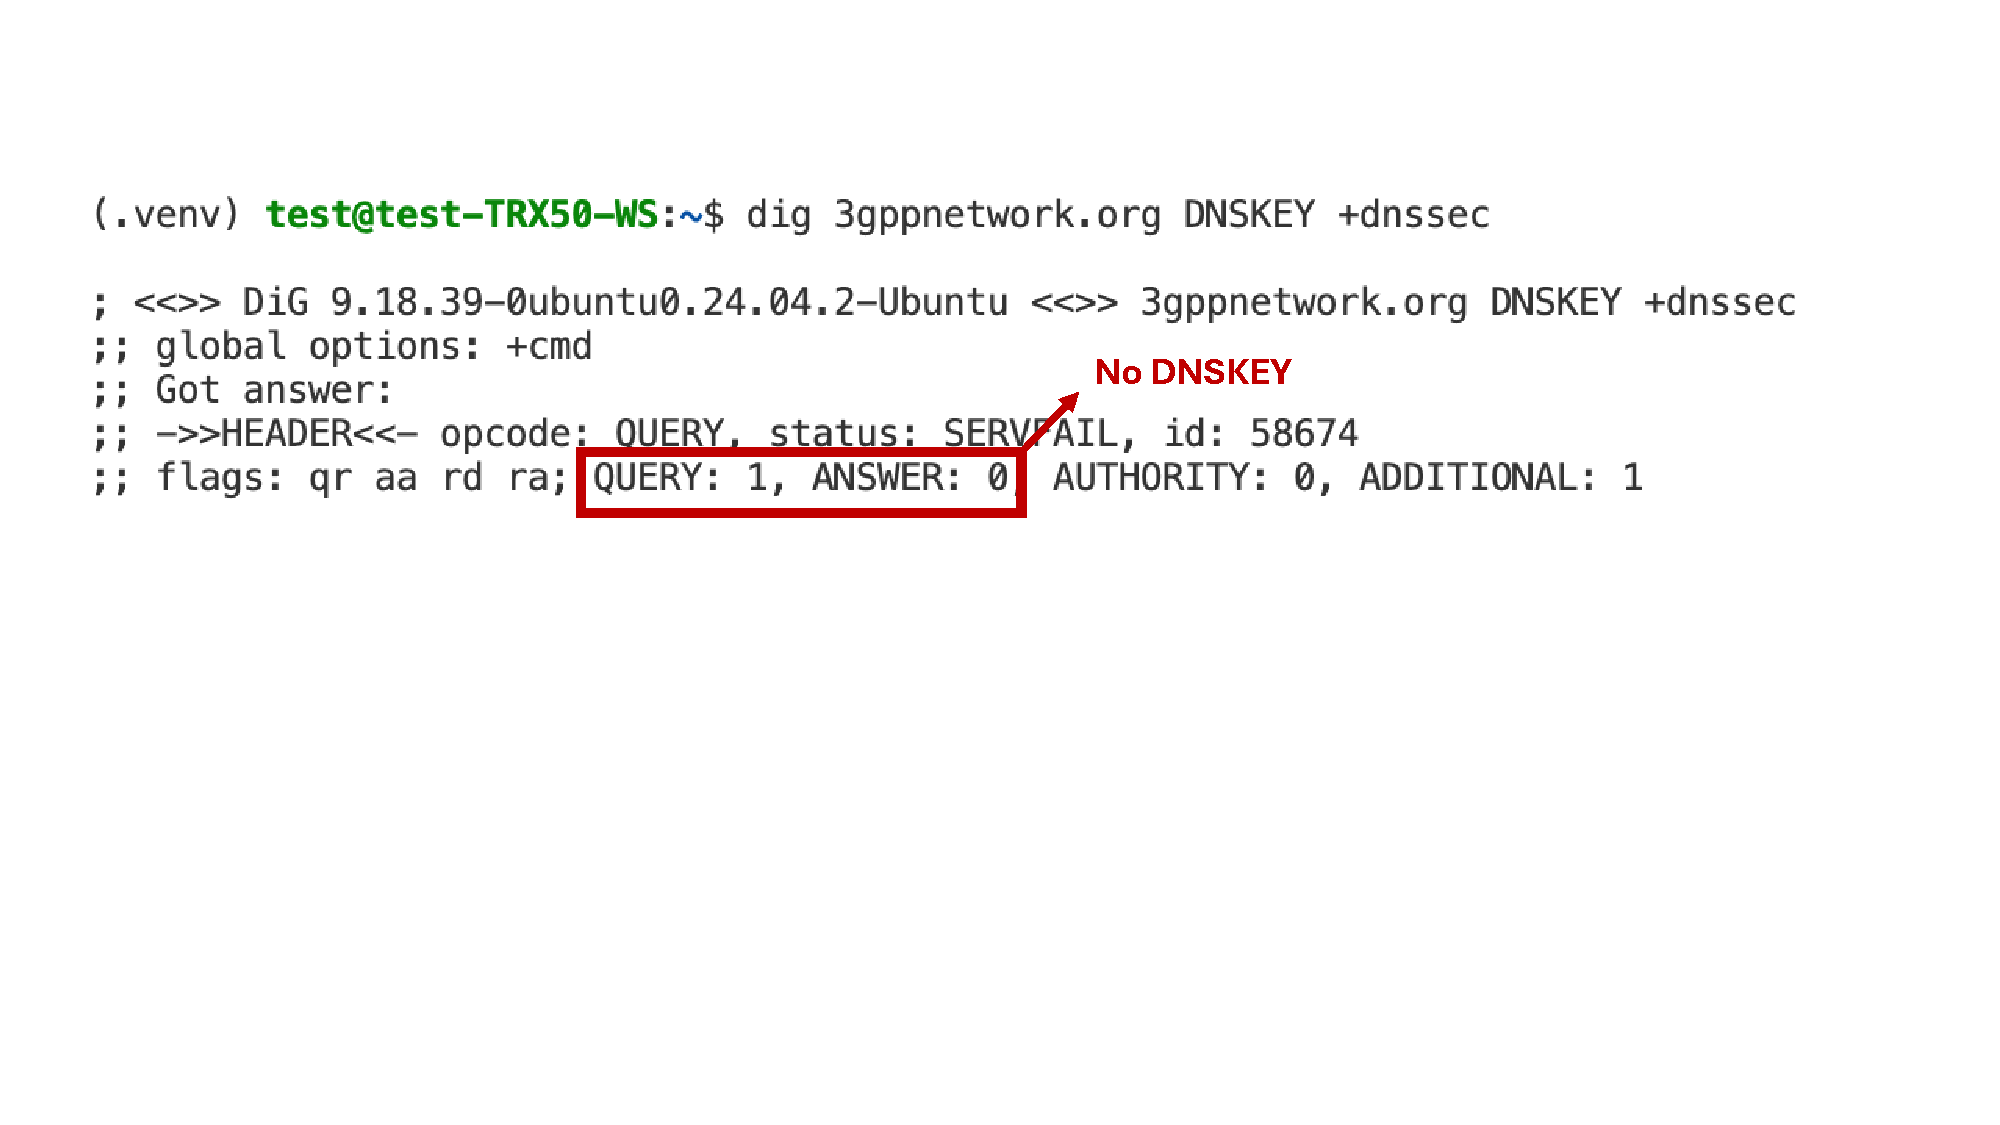
\includegraphics[width=0.9\linewidth]{pic/dig-commend.pdf}
    \vspace{-0.15in}
    \caption{`3gppnetwork.org' does not enable DNSSEC}
    \label{fig:dig-command}
    \vspace{-0.2in}
\end{figure}

For (1), we first test whether the parent domain `3gppnetwork.org', managed by GSMA, is protected by DNSSEC, because DNSSEC validation for any descendant name (e.g., DNS-based PLMN Discovery) relies on a valid chain of trust. 
 
Our measurement via the tool \texttt{dig}~\cite{isc-bind}, as shown in Figure~\ref{fig:dig-command}, indicates that the DNSSEC for `3gppnetwork.org' is absent. 
Therefore, DNS-based PLMN discovery remains vulnerable to classic DNS manipulation threats on untrusted links, even when subsequent procedures are cryptographically protected.  

For (2), to evaluate whether the DNS manipulation can work, we test whether a poisoned discovery response can prevent the UE from establishing a secure tunnel to the legitimate N3IWF. 
Since conducting Internet-scale poisoning experiments is unethical, we perform experiments in a controlled environment. 
Specifically, we use two COTS UEs, Samsung S24 and Moto G Stylus 5G on T-Mobile network, and connect them to a controlled Wi-Fi router configured to poison DNS queries relevant to `3gppnetwork.org'. After enabling Wi-Fi calling services, we observe that both UEs try to resolve the IP address of N3IWF (i.e., ePDG for Wi-Fi calling services). 
Under the poisoned resolution, the UEs attempt to connect to the misdirected endpoint, thereby preventing the UE from reaching the legitimate N3IWF and completing non-3GPP access registration. This shows that, even though subsequent N3IWF procedures provide cryptographic protection and mutual authentication, compromising the discovery stage can still induce a denial-of-service attack.  

\subsubsection{Root Cause and Lesson Learned.} The root cause is a trust gap in the DNS-based PLMN discovery, which is performed over untrusted access links before the UE establishes a secure channel to the operator's infrastructure. 
It is a standard design flaw that 3GPP specifications only protect the post-discovery connection and do not enforce security mechanisms during the discovery stage, which allows adversaries to exploit unauthenticated discovery to misdirect the victim.  
To address this vulnerability, future 3GPP specifications must enforce the security mechanisms on DNS-based PLMN discovery in two ways. First, discovery infrastructure must be treated as security-critical. Operational domains used for standardized discovery must provide an authenticated naming and resolution path. Second, standards need to mandate a robust fallback mechanism that avoids futile attempts.  

\begin{figure}[t]
    \centering
    \includegraphics[page=4,width=0.8\linewidth]{pic/New_Vulnerabilities.pdf}
    \vspace{-0.15in}
    \caption{Privacy Exposure via Over-Disclosed VoIMS Signaling Headers}
    \label{fig:privacy_exposure}
    \vspace{-0.2in}
\end{figure}


\subsection{V4: Privacy Exposure via Over-Disclosed VoIMS Signaling Headers} 

\noindent With the introduction of the all-IP network architecture in 4G LTE, call services previously supported by conventional circuit-switched (CS) technology in legacy 2G/3G networks have transitioned to being provided by the IMS. To facilitate IMS-based call services (also known as VoIMS - Voice over IMS), the Session Initiation Protocol (SIP), widely used in voice over IP services, was adopted for call signaling, replacing the legacy CS Call Control (CC) protocol. SIP is a text-based, string-oriented protocol, in contrast to the binary, structure-oriented CS CC protocol. 

Adopting a text-based call signaling protocol is a double-edged sword. While it offers greater flexibility and extensibility to support various emerging IP-based multimedia services compared to conventional protocols, it also introduces new issues due to potential missteps in design. Specifically, all 2G/3G CC signaling messages are designed to carry specific 3GPP-stipulated content only. In contrast, the text-based SIP protocol allows carriers and mobile devices to transmit a much broader range of content. 
Specifically, TS~24.229 stipulates 113 SIP headers and 15 SDP headers to support IMS-based call services, far more than its predecessor. These IMS service signaling headers can carry personal, device, and infrastructure details. 

Unfortunately, as shown in Figure \ref{fig:privacy_exposure}, there are no privacy preservation mechanisms enforced in 3GPP specifications for IMS signaling headers. While the signaling messages for normal IMS services are encrypted by IPSec, operators and UEs would carry such privacy-exposing headers to both IMS service users who can be the adversaries who collect the privacy information that may enable subsequent attacks.  



\subsubsection{Experimental Validation.} We validate this potential privacy leakage by examining privacy leaks during call interworking. We control 2 phones, a Samsung S21 and a Google Pixel 5, on three US carriers (labeled as OP-I, OP-II, and OP-III) and collected signaling messages exchanged between two call ends. We make 10 calls for each combination of phone model and carrier. Our experimental results show that on the operational IMS services, privacy-leaking headers are transmitted and received by the UEs. Two privacy issues are explicitly identified in the messages SIP INVITE and SIP SESSION PROGRESS. In the former, as shown in Figure~\ref{fig:user-agent}, it is observed that the caller's User-Agent header is transmitted to the callee through the OP-II network, leaking the phone model and security patch version to the callee. For the latter as shown in Figure~\ref{fig:name-server}, when the caller is on OP-III, and the callee is on OP-I, P-Asserted-Identity and Server headers are added by the networks in the SIP SESSION PROGRESS response, revealing the callee's identity and IMS server information. 

\begin{figure}[t]
    \centering
    \begin{subfigure}[b]{0.45\textwidth}
        \centering
        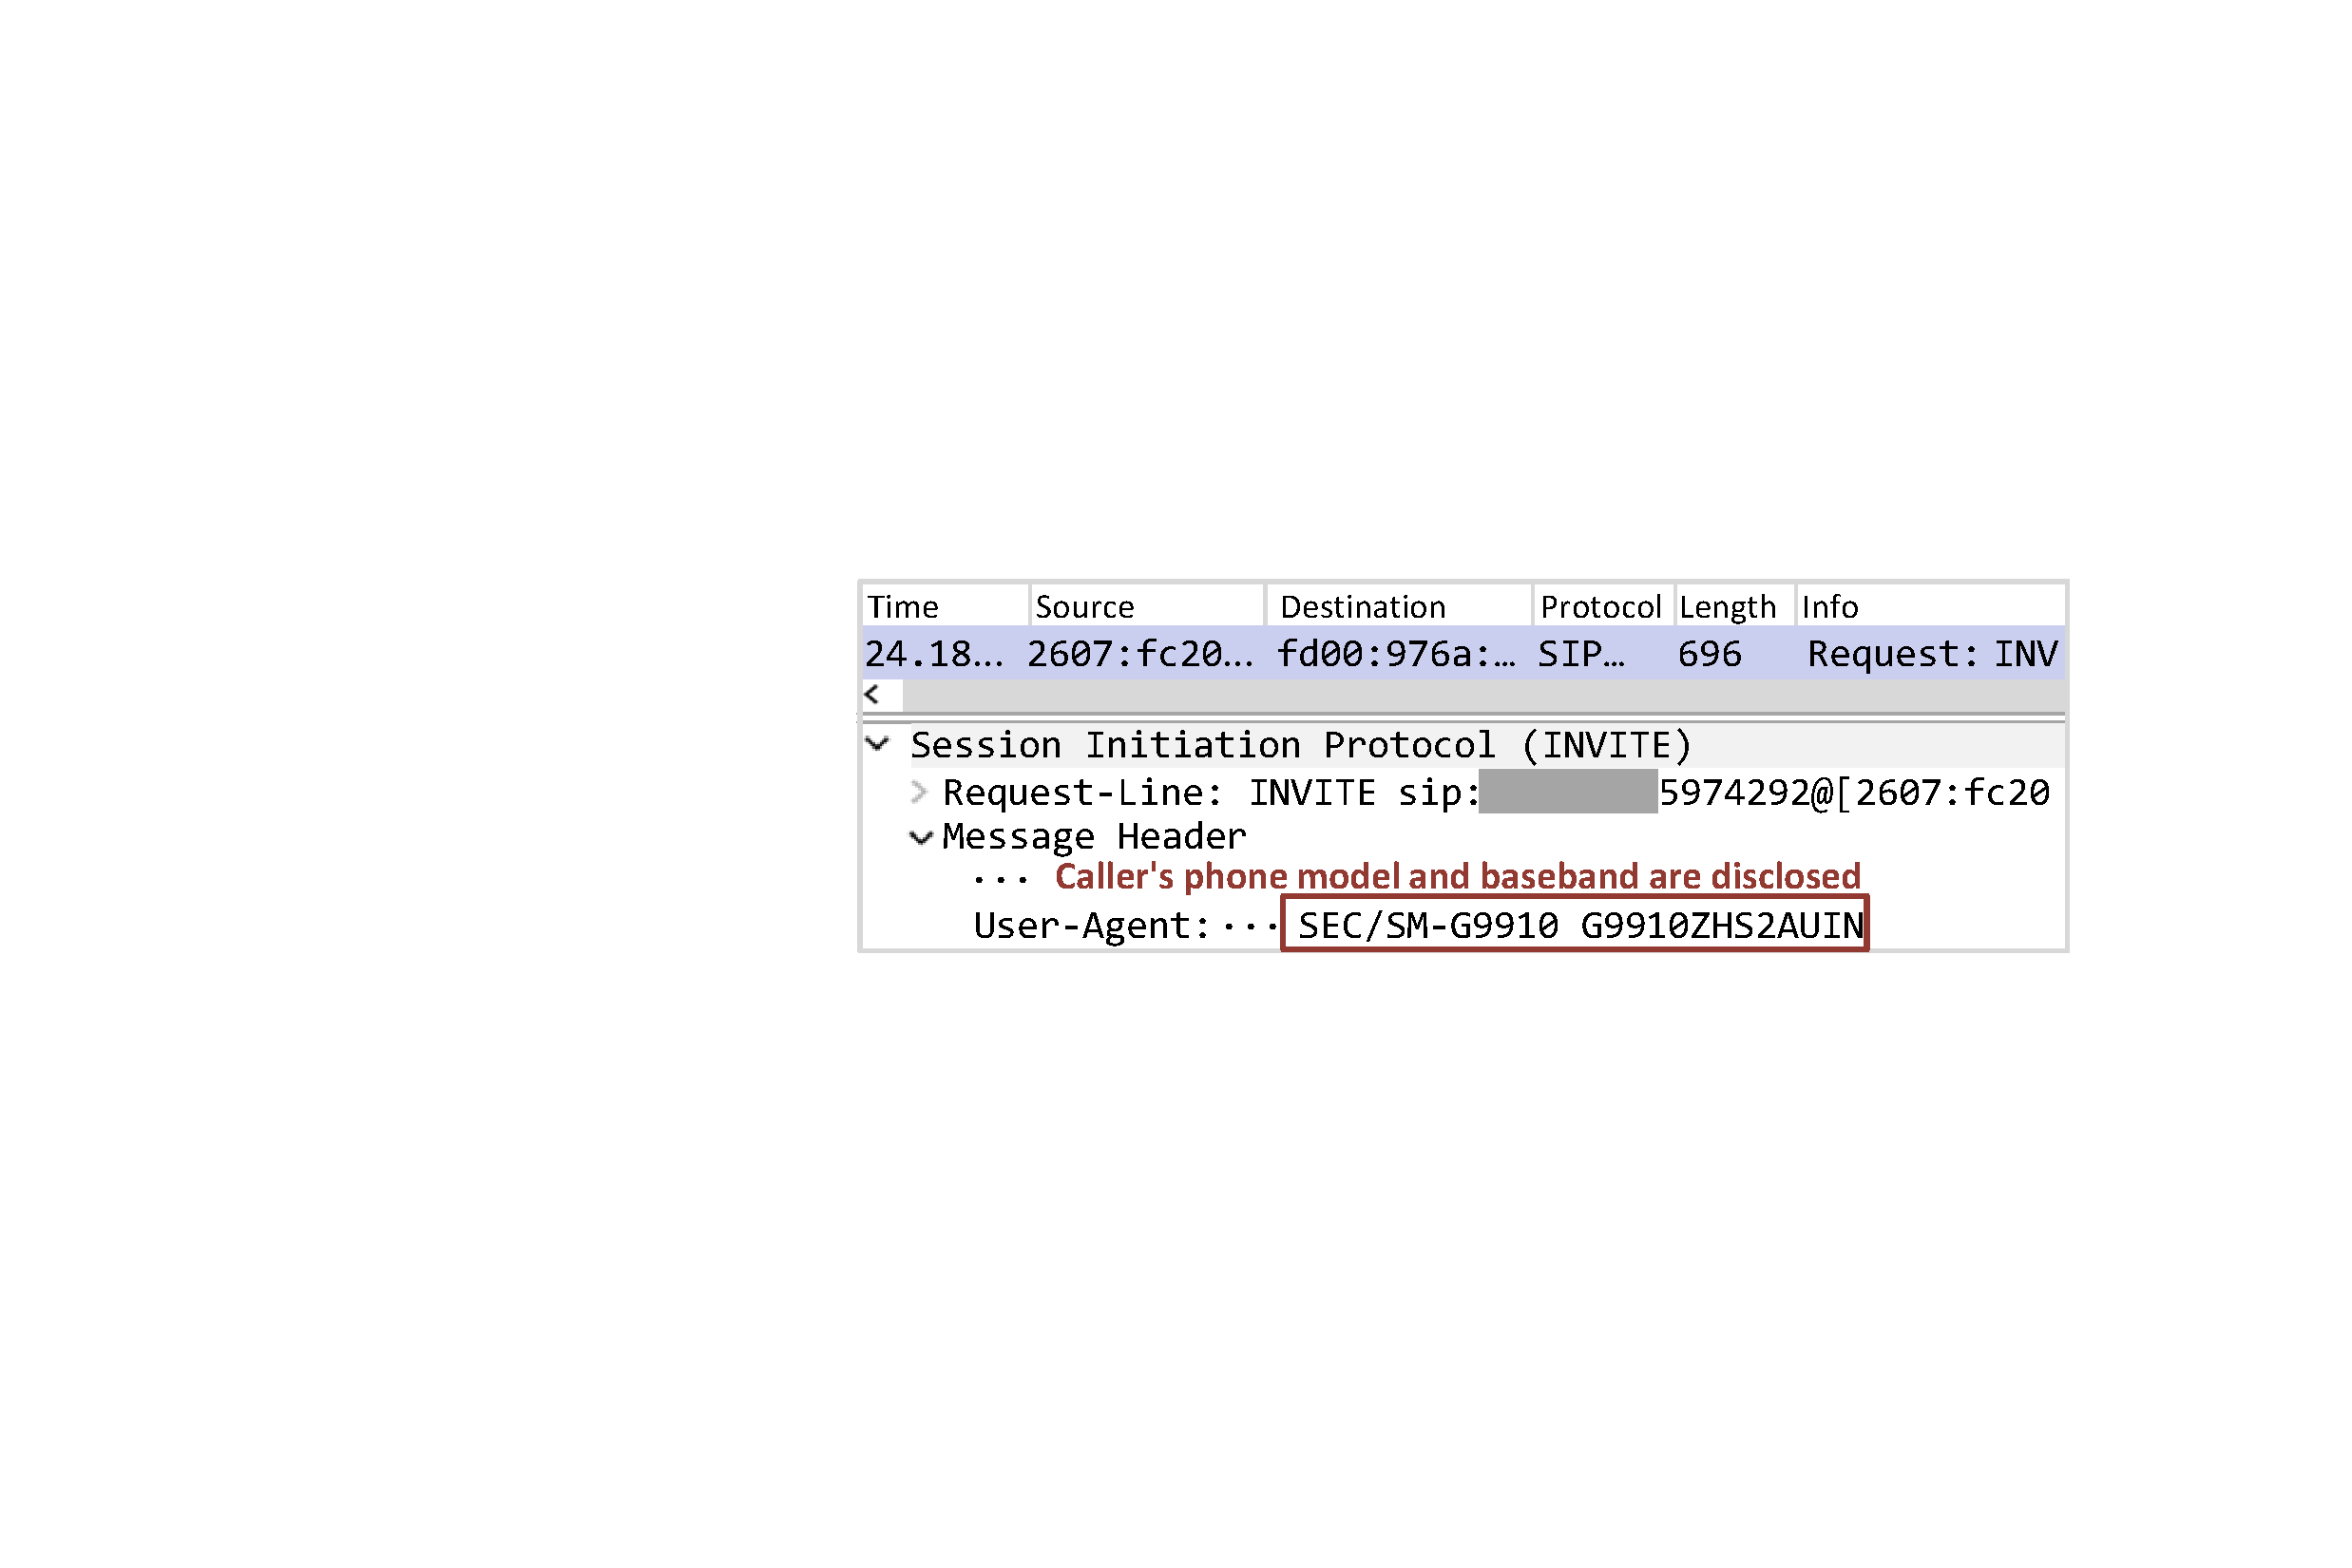
\includegraphics[width=\textwidth]{pic/privacy-leak-phone-model.pdf}
        \caption{User-Agent header leaks phone model and security patch version}
        \label{fig:user-agent}
    \end{subfigure}
    \hfill
    \begin{subfigure}[b]{0.45\textwidth}
        \centering
        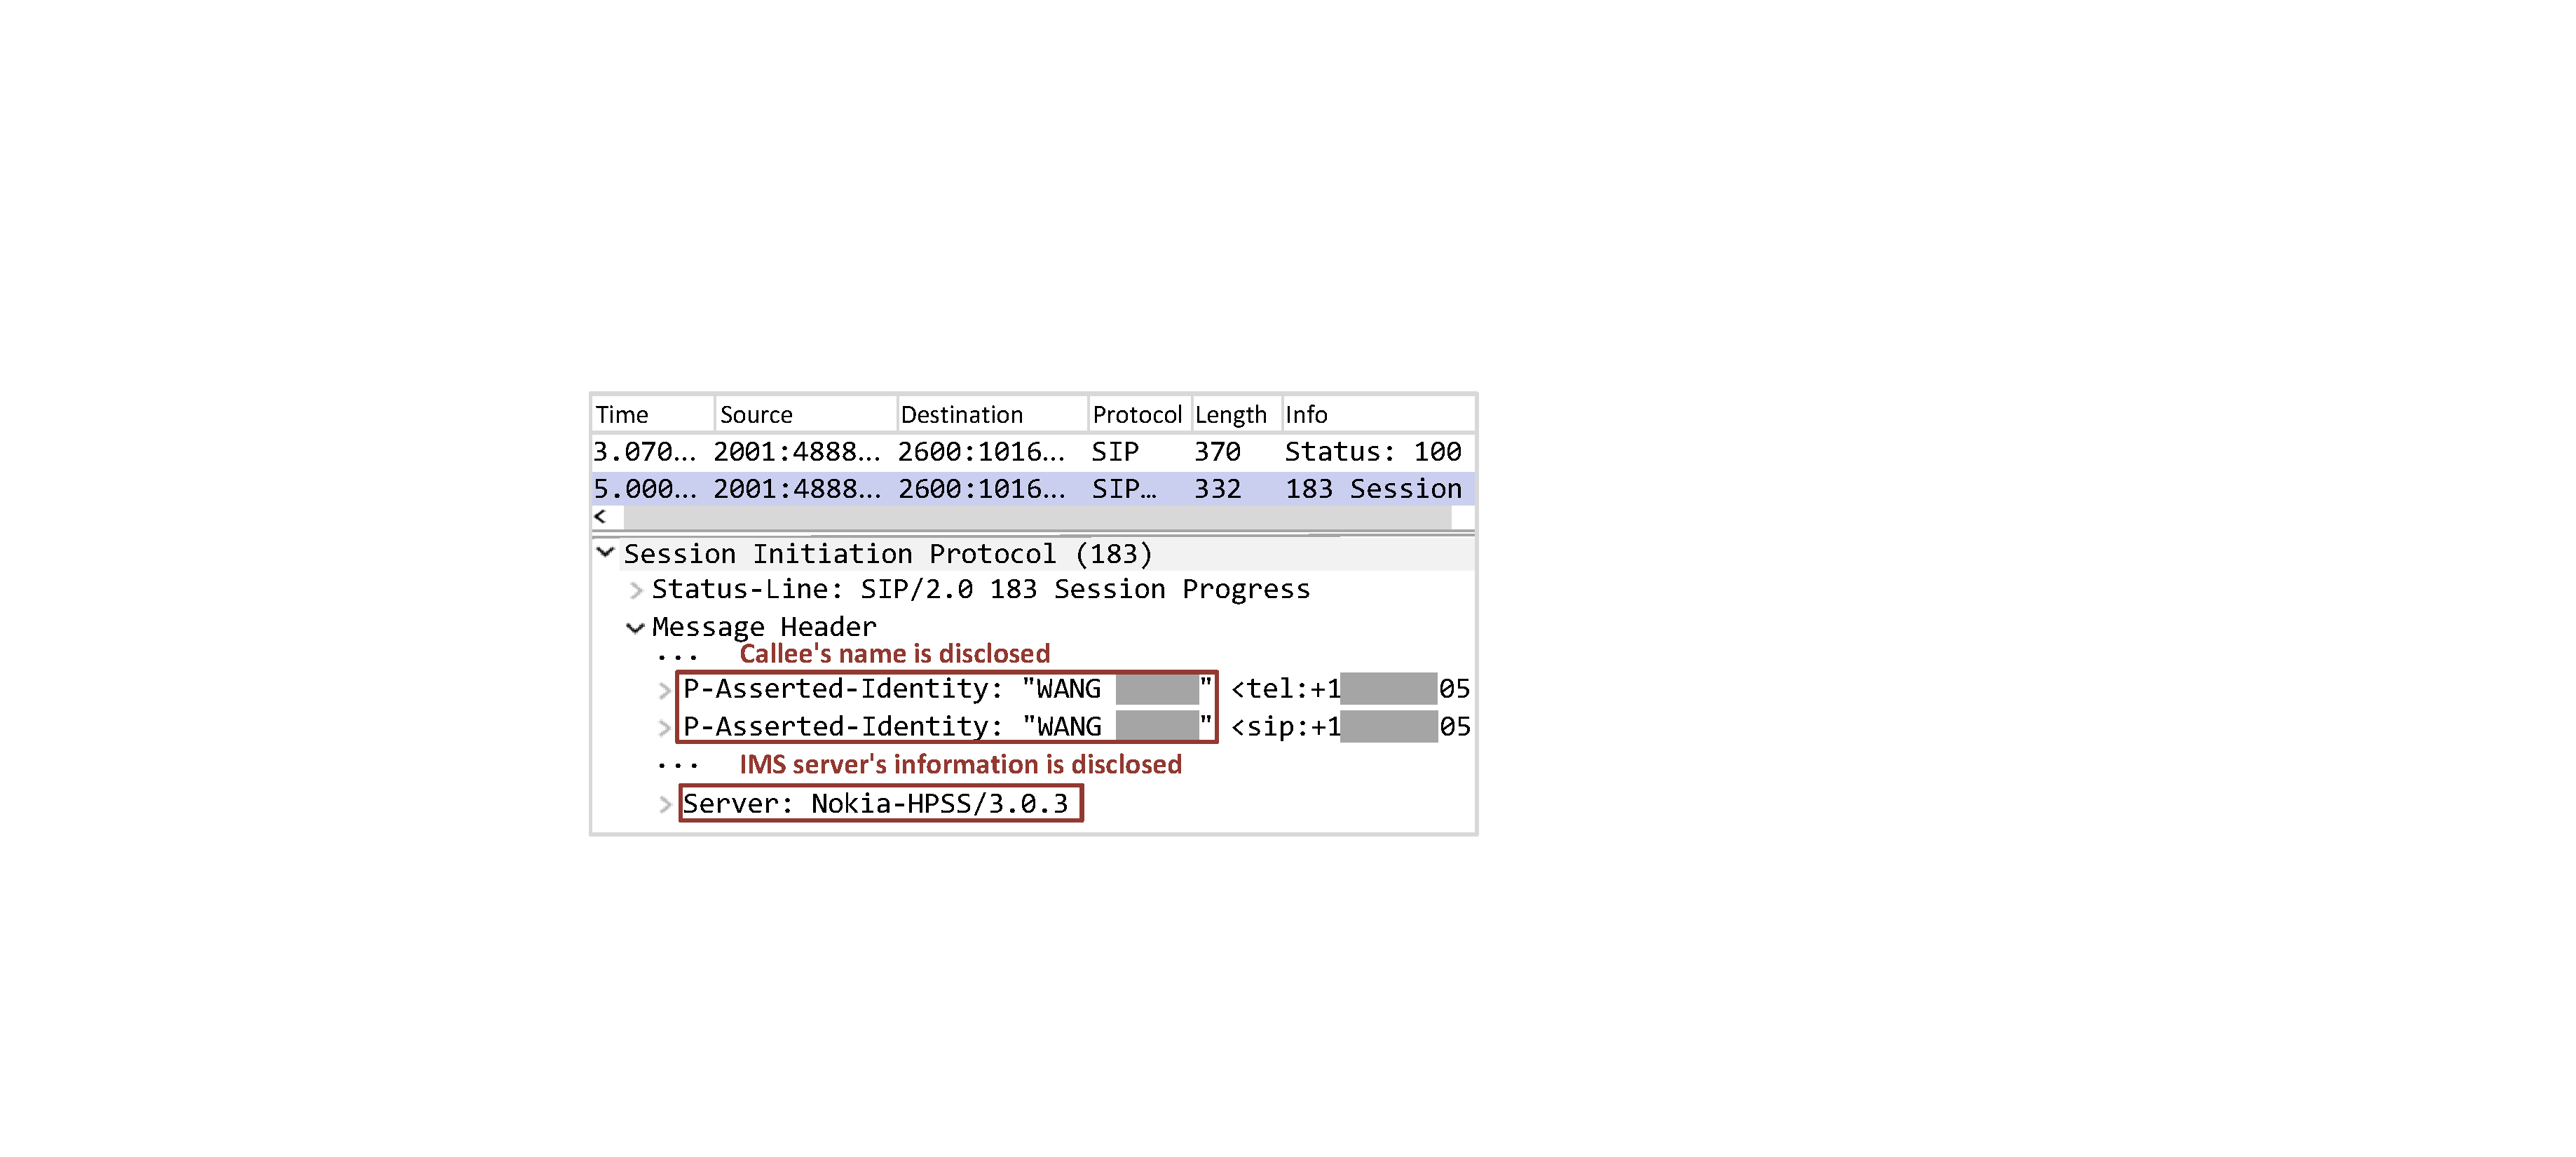
\includegraphics[width=\textwidth]{pic/privacy-leak-name-server.pdf}
        \caption{P-Asserted-Identity and Server headers leak callee's name and IMS server's information}
        \label{fig:name-server}
    \end{subfigure}
    \vspace{-0.1in}
    \caption{The information about users and cellular infrastructure is leaked during call interworking}
    \label{fig:main}
    \vspace{-15pt}
\end{figure}


\subsubsection{Root Cause and Lesson Learned.} Adopting a text-based call signaling protocol allows carriers and mobile devices to transmit a much broader range of content. While the 3GPP specification does not prohibit the transmission of these abundant headers, other network standard organizations like the IETF have raised concerns about privacy risks from unnecessary header disclosures. For example, RFC 3261~\cite{RFC3261} warns about the vulnerability of disclosing user agent information. This underscores the urgent need for 3GPP to review and revise its IMS-related specifications with a focus on privacy preservation. 



\subsection{V5: Exploitable CS-Fallback Initiation} 

\begin{figure}[t]
    \centering
    \includegraphics[page=5,width=0.8\linewidth]{pic/New_Vulnerabilities.pdf}
    \vspace{-0.15in}
    \caption{Exploitable CS-Fallback Initiation}
    \label{fig:csfallback}
    \vspace{-0.2in}
\end{figure}

\noindent 4G LTE networks support Circuit-Switched Fallback (CSFB) to provide legacy CS voice/SMS by redirecting a UE to a CS network (e.g., 2G/3G if available) when VoLTE is unavailable. 
Note that 5G non-standalone deployments that rely on 4G LTE infrastructure also support CSFB.   
In CSFB, after a UE in EMM-IDLE receives a paging request for a CS service, it initiates fallback by sending an EXTENDED SERVICE REQUEST to the Core Network. In the common case, the UE transitions from RRC\_IDLE to RRC\_CONNECTED and sends this request as an initial NAS message. In this case, the initial message is only integrity-protected without ciphering because NAS ciphering is only applied after the access-stratum connection and the relevant security context are re-activated for this specific exchange. Thus, adversaries can sniff the \textsf{EXTENDED SERVICE REQUEST}. 

Moreover, TS~24.301 allows certain NAS reject messages, including SERVICE REJECT, to be sent and processed without any security protection. This combination exposes a practical CSFB DoS attack surface: adversaries can deny CSFB and rate-limit subsequent attempts by (1) sniffing unciphered EXTENDED SERVICE REQUEST and (2) injecting forged SERVICE REJECT with EMM cause \#39 (CS domain temporarily not available) and the associated timer T3442 to throttle subsequent attempts. 



\subsubsection{Proof-of-concept Attack.} Figure~\ref{fig:csfallback} illustrates a proof-of-concept attack. The attacker deploys a sniffer between the victim and the legitimate eNodeB. Once an unciphered EXTENDED SERVICE REQUEST is observed, the attacker immediately sends a forged SERVICE REJECT carrying EMM cause \#39 and the T3442 via a rogue base station.  
To validate this attack, as shown in Figure~\ref{fig:device-setup}, we implement an SDR-based testbed using srsRAN and open5GS~\cite{open5gs}, both of which support CS Fallback. 
A Samsung S24 and a Moto G Stylus are used as test UEs. Instead of building a full injection pipeline that monitors unciphered NAS messages and injects forged responses, which are credited to prior works~\cite{hussain2018lteinspector}, we simplify the evaluation by configuring Open5GS and srsRAN to emulate a CS call paging and then directly respond with a SERVICE REJECT with EMM cause \#39 and T3442 for the maximum value 30 mins directly. 
As shown in Figure~\ref{fig:csfb}, the experimental traces indicate that the UEs accept the rejection and stop attempting to set up the call. 
Overall, this attack achieves a stealthy denial-of-service against CS services on LTE by preventing a CSFB procedure, and limiting further CSFB attempts via \textsf{T3442}. The throttling effect is particularly damaging because the UE self-enforces the backoff timer. Depending on UE implementation and timer configuration, the victim may experience prolonged inability to place CS calls. We leave a systematic characterization of the maximum outage duration to future work.   


\begin{figure}[t]
    \centering
    \includegraphics[page=5,width=0.8\linewidth]{pic/testd.jpeg}
    \vspace{-0.15in}
    \caption{The setup for validating V5: Exploitable CS-Fallback Initiation}
    \label{fig:device-setup}
    \vspace{-0.2in}
\end{figure}



\begin{figure}[t]
    \centering
    \includegraphics[page=5,width=0.95\linewidth]{pic/cs-fallback.jpg}
    \vspace{-0.15in}
    \caption{The victim UE accepts the rejection and ceases its attempts to establish the call}
    \label{fig:csfb}
    \vspace{-0.2in}
\end{figure}


\subsubsection{Root Cause and Lesson Learned.} The root cause is TS~24.301 explicitly permits a SERVICE REJECT to be processed without ciphering and integrity protection. This design appears risky but serves as a fail-safe mechanism for cases where a secure connection cannot be established or has been lost. For example, if a UE sends an EXTENDED SERVICE REQUEST but the MME cannot authenticate the user (e.g., the unknown/invalid subscription), the network must be able to instruct the UE to stop trying without security keys. Similarly, for emergency services, the network must always be able to reject or redirect requests even if security procedures are failing to ensure the UE can seek alternative access. 
To mitigate this threat, commonly from rogue base stations, and still allow certain unprotected signaling messages for a fail-safe mechanism, in practice, it likely requires UE-side defenses against rogue base stations and stricter validation before setting the long throttling timers. 



\subsection{V6: Access Trap via Access Barring Factor} 


\noindent In 5G NR, System Information Block 1 (SIB1) is a periodically broadcast RRC message that every UE must decode first before any AS (Access Stratum) security is established. SIB1 carries essential cell-access and cell-selection parameters, including PLMN, scheduling of other system information blocks, and uac-BarringInfo for UAC (User Access Control). uac-BarringInfo specifies barring rules for different access categories, distinguishing everyday services (e.g., regular voice/data and mobile-originated signaling) from special-case/high-priority categories (e.g., paging/mobile-terminated access and emergency access). A similar design also existed in 4G networks, which used the ac-BarringInfo field in SIB2 messages.

Each barring rule includes parameters such as barringFactor, which controls the probability that a UE is allowed to initiate an access attempt for a given category. Intuitively, a smaller barringFactor imposes a stronger restriction, while an extremely small value can cause most or nearly all UEs to defer their mobile-originated requests. In normal operation, base stations typically configure moderate barring parameters, or disable barring entirely, to preserve broad service availability and avoid unnecessarily suppressing legitimate access.


This design becomes exploitable when a malicious base station advertises an extremely restrictive barringFactor in SIB1/SIB2 in 5G/4G networks. After decoding the broadcast information, the UE enforces the barring policy locally. By setting barringFactor to a highly restrictive value, the attacker can effectively drive victim UEs into a stealthy nonfunctional state, where the device appears camped on a cell but repeatedly refrains from initiating normal services, thereby creating a stealthy denial-of-service condition. 


\begin{figure}[t]
    \centering
    \includegraphics[page=6,width=0.8\linewidth]{pic/New_Vulnerabilities.pdf}
    \vspace{-0.15in}
    \caption{Access Category Trap via SIB1 Access Barring}
    \label{fig:sib1}
    \vspace{-0.2in}
\end{figure}

\subsubsection{Proof-of-concept Attack.} Figure~\ref{fig:sib1} illustrates the proof-of-concept attack. The adversary only needs to operate a rogue base station and exploit broadcast system information; no cryptography is broken. Specifically, the adversary needs to configure the rogue base station to broadcast SIB1 in 5G/SIB2 in 4G with barringFactor set to a highly restrictive value (e.g., 0), which sets a low probability that a UE is allowed to initiate an access attempt. Therefore, any nearby UEs that receive and decode this SIB1/SIB2 are not able to initiate an access attempt. 



To validate this vulnerability ethically, we implement an SDR-based testing platform using srsRAN and srsEPC. All antennas are placed in a shield box to ensure that no unintended over-the-air transmissions occur.
We use a Samsung S24 and a Moto G Stylus 5G as test phones. 
Next, we simplify the experiment and configure the controlled serving cell to broadcast SIB2 with an ac-BarringFactor setting to 0. As shown in Figure~\ref{fig:sib2}, we observe (i) the UE does not initiate RRC connection establishment after receiving a SIB2 with BarringFactor setting to 0, and (ii) the data service on UEs is not usable without interfaces. Our experimental results show that both phones self-block service without explicit alerting beyond generic `no service' icon, consistent with the intended UAC enforcement behavior but enabling a stealthy denial-of-service. 


\begin{figure}[t]
    \centering
    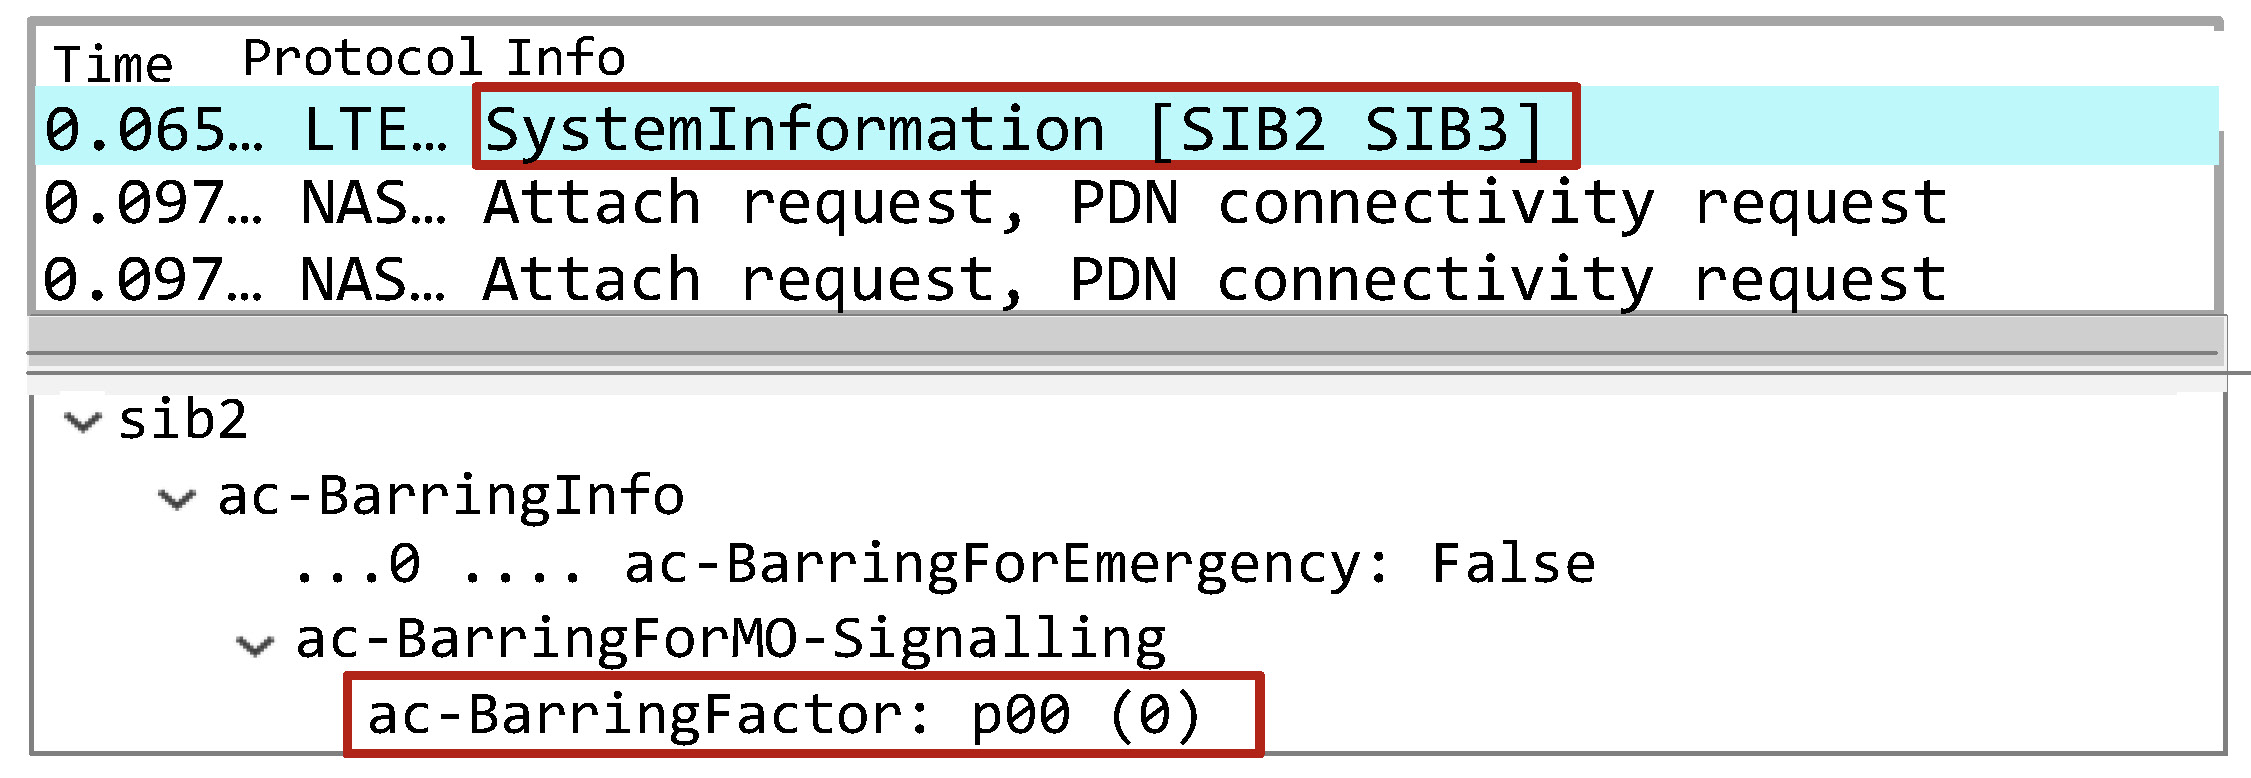
\includegraphics[width=0.95\linewidth]{pic/sib2.jpg}
    \vspace{-0.15in}
    \caption{The SIB2 messages broadcast by attackers prevent UEs from attaching to base stations}
    \label{fig:sib2}
    \vspace{-0.2in}
\end{figure}


\subsubsection{Root Causes and Lesson Learned.} UAC is designed for congestion control: the UE locally enforces access restrictions to reduce network load and stabilize access attempts during overload. However, the policy is delivered via SIB1/SIB2, which is broadcast and processed prior to authentication and therefore lacks integrity protection. This creates a pre-authentication trust gap: a rogue cell can advertise restrictive UAC policies and rely on the UE to self-enforce them, achieving denial-of-service without needing to defeat cryptographic protections.
To mitigate this vulnerability, 3GPP standards shall develop UE implementations that can reduce exposure by adding safety checks and recovery logic (e.g., bounding the duration of extreme barring, triggering reselection/blacklisting when a newly camped cell persistently bars most categories, or cross-validating with neighboring cells). 




\subsection{V7: Rogue Base Station RRC RESUME Blackhole}

\noindent In 5G NR, a UE selects the cell based on the broadcast radio information and measured radio conditions before any AS/NAS security context is activated. Concretely, parameters conveyed via the broadcast messages (e.g., SSB/PBCH, MIB, and SIBs) are not authenticated at the UE during this procedure. As a result, a rogue base station can attract a UE through (1) stronger radio conditions in terms of RSRP, RSRQ, and SINR, (2) advertising the legitimate PLMN info that the UE is willing to use, and (3) advertising that it is not barred for achieving a high priority in the standard cell selection and reselection mechanism defined in TS~36.304.

Combining the cell selection and reselection mechanism with the RRC RESUME procedure that a UE in RRC INACTIVE expects to resume quickly via RRC RESUME REQUEST, the UE can be induced to reselect into a gNB that does not recognize or even a rogue gNB that can intentionally ignore or reject this request. 
This resume thus fails. Moreover, instead of directly switching to another cell, TS~36.304~\cite{3gpp_ts36304} defines that a UE should retry after a wait time specified by the timer T302. The cell selection and reselection mechanism does not consider the resume failure. Thus, the victim UE will stick to the malicious base station until a legitimate gNB wins in the cell selection and reselection procedure. 
While 5G security prevents a rogue gNB from completing an authenticated service, repeated resume failures can still cause meaningful availability harm for the retry loops. 


\begin{figure}[t]
    \centering
    \includegraphics[page=7,width=0.8\linewidth]{pic/New_Vulnerabilities.pdf}
    \vspace{-0.15in}
    \caption{Rogue Base Station RRC RESUME Blackhole}
    \label{fig:rrcresume_blackhole}
    \vspace{-0.2in}
\end{figure}

\begin{table*}[!t]
\centering
\caption{Comparison of existing systems for 3GPP specification security analysis}
\label{tab:spec-compare}
\vspace{-0.1in}
\scriptsize
\begin{tabular}{p{1.8cm} p{3cm} >{\centering}p{1.8cm} p{2.8cm} p{6cm}}
% \begin{strip}
% \centering
% \captionof{table}{Comparison of existing systems for 3GPP specification security analysis}
% \label{tab:spec-compare}
% \scriptsize
% \begin{tabular}{p{1.8cm} p{3cm} >{\centering}p{1.8cm} p{2.8cm} p{6cm}}
\toprule
\textbf{Method} & \textbf{Primary Objective} & \textbf{Protocol Modeling} & \textbf{Security Scope} & \textbf{Remarks} \\
\midrule

\textbf{Atomic}~\cite{chen2021bookworm} &
Detecting hazard indicators via textual entailment &
\xmark &
Risk‐sentence detection only &
Identifying hazard indicators via sentence-level textual entailment without modeling specification logic or performing systematic vulnerability analysis \\


\midrule

\textbf{ConTester}~\cite{chen2023sherlock} &
Extracting security requirements &
\xmark &
Developing conformance test cases &
Only extracting security requirements for developing conformance test without uncovering design-level vulnerabilities \\


\midrule

\textbf{CellularLint}~\cite{rahman2024cellularlint} &
Detecting semantic inconsistencies &
\xmark &
Sentence‐level contradiction detection &
Detecting semantic inconsistencies (i.e., sentence-level contradictions) via sentence-pair inference instead of reasoning over complete specification logic \\

\midrule

\textbf{Hermes}~\cite{al2024hermes} &
Automatic FSM extraction via traditional NLP approaches &
\cmark &
Formal security analysis &
Parsing specifications via handcrafted grammars using constituency parsing and dependency parse trees, remaining rule-intensive and lacking flexibility to adapt to evolving specifications \\

\midrule

\textbf{ARCANE}~\cite{tan2025automated} &
Automated vulnerability discovery via model-based fuzzing &
\cmark &
Implementation vulnerability discovery &
Automatically constructs protocol models and performs model-based fuzzing \\

\midrule

\textbf{\lm } &
End‐to‐end SCA nodes and systematic vulnerability reasoning &
\cmarkbold &
Specification‐level design‐flaw detection &
First system to enable scalable specification extraction and systematic security analysis \\

\bottomrule
\end{tabular}
\end{table*}
% \end{tabular}
% \end{strip}



\subsubsection{Proof-of-concept Attack.} 
We refer to the following behavior as an \emph{RRC RESUME Blackhole}: the victim UE is trapped within a rogue gNB and stuck in repeated RRC RESUME REQUEST$\rightarrow$\ RRC RESUME failure cycles. 
The attacker does not need to break cryptography and does not need to complete mutual authentication. Instead, the attacker exploits (i) unauthenticated cell selection and (ii) the coupling between reselection and the RRC RESUME mechanism. 

\begin{figure}[H]
    \centering
    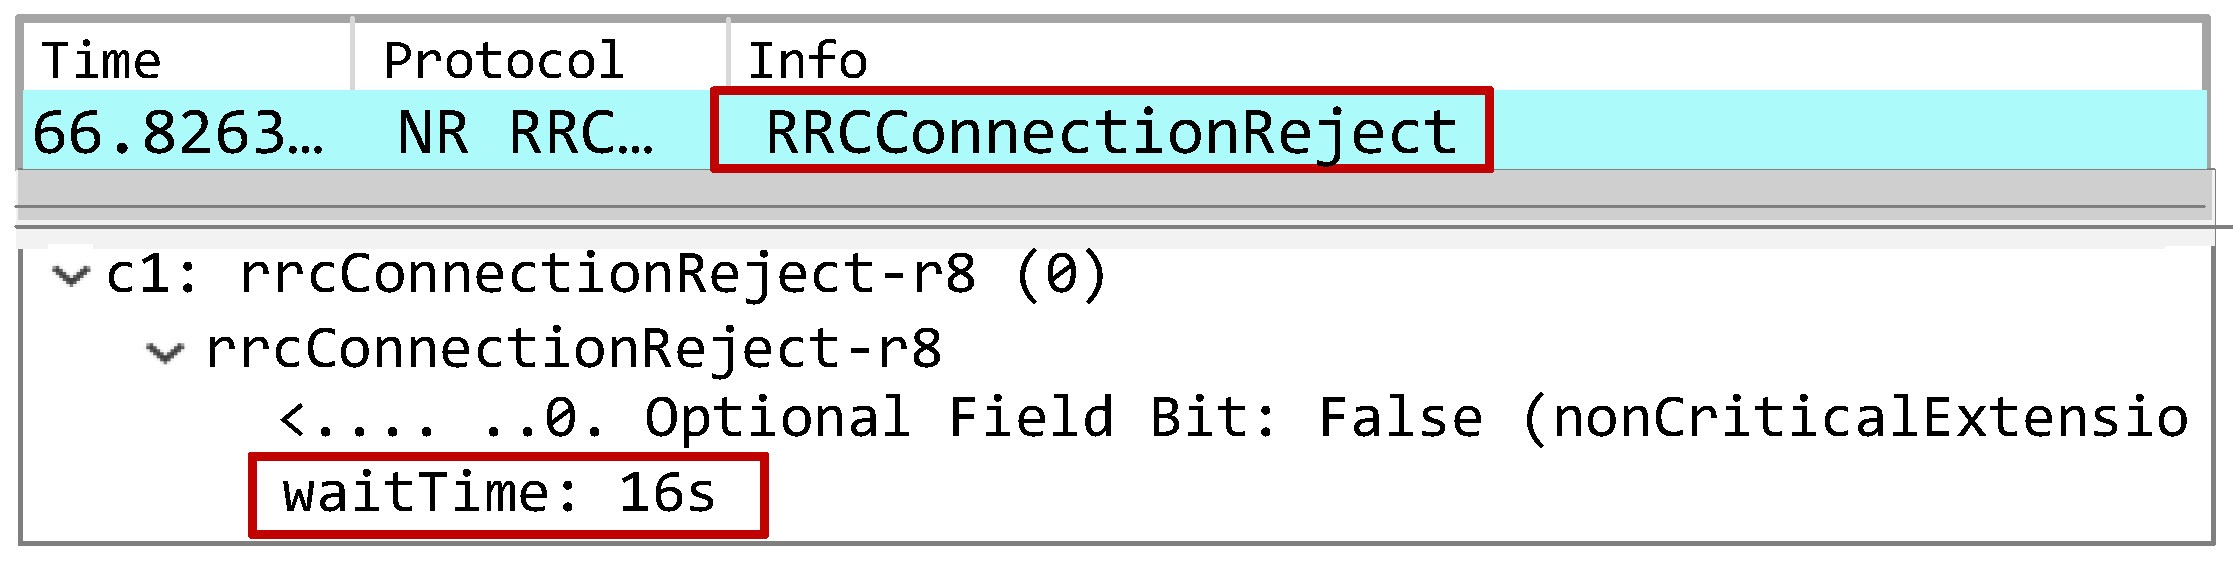
\includegraphics[width=0.95\linewidth]{pic/rrcresume.jpg}
    \vspace{-0.05in}
    \caption{The victim UE remains unable to resume services and repeats the procedure every 16 seconds according to the timer.}
    \label{fig:timer}
    \vspace{-0.2in}
\end{figure}


For ethical reasons, we validate this attack in a fully controlled environment. First, inside an RF shield box, we deploy two SDR-based gNBs using srsRAN and open5GS: One serves as a legitimate gNB, and another serves as the rogue gNB. The rogue gNB is configured to have same settings as the legitimate one. Two test phones, a Samsung S21 and a Moto G Stylus 5G, are employed. Second, we increase the rogue gNB signal strength via increasing its tx\_gain and rx\_gain in srsRAN so that the rogue gNB can be the first choice in the cell selection and reselection mechanism. Third, we operate the test phones to trigger the RRC RESUME. Fourth, we configure the rogue gNB to respond with RRC REJECT for all RRC RESUME REQUEST with a RejectWaitTime 16, which will be the time used by the UE as T302. Last, we examine if the UE is stuck to the rogue gNB and trapped within RRC RESUME Blackhole. Figure~\ref{fig:timer} illustrates a trace captured on the Moto G Stylus 5G, which remains unable to resume service for 16 seconds after receiving RRC REJECT. The Samsung S21 exhibits a different implementation behavior: it does not strictly follow the 3GPP-specified wait time and stops sending RRCResumeRequest for only about 3 seconds even when RejectWaitTime $=$ 16 is provided. This result shows that although the attack is effective on both devices, UE implementations may differ in how strictly they enforce the backoff timer.



\subsubsection{Root Causes and Lessons Learned.} The root cause is that the cell selection and reselection mechanism developed in 3GPP standards does not consider these failures. It operates on the RRC layer before the UE can establish a protected AS channel. Future specifications and deployments can consider additional mechanisms to reduce resume failures (e.g., explicit guidance for UEs to switch from cells that cannot support resumption). 




\vspace{-5pt}

\section{Related Work}
\label{append:Related_Work}
Table \ref{tab:spec-compare} summarizes and contrasts representative 3GPP specification analysis systems in terms of their primary objectives, protocol modeling capabilities, security analysis scope, and key methodological characteristics.



\section{\textit{\lm}}
\label{append:prompt_algorithm}
This appendix provides implementation-level details of the prompts and algorithms used by \lm. It covers \textit{SpecAdaptation}, the \textit{SCA Representation Extractor}, the \textit{Function Chain Builder}, \textit{SecOracle}, and \textit{VulnTestGenerator}. The Function Chain Builder is formalized through Algorithm~\ref{alg:temporal_connection}, Algorithm~\ref{alg:semantic_connection}, Algorithm~\ref{alg:causal_connection}, and Algorithm~\ref{alg:reference_connection}, which respectively define Temporal, Semantic, Causal, and Reference Guided Connection.

\subsection{SpecAdaptation}

\vspace{-5pt}

\begin{algorithm}[ht]
\caption{\textit{SpecAdaptation}}
\label{alg:rag_prompt}
\scriptsize
\begin{algorithmic}[1]

\State \textbf{Input:} Versioned 3GPP corpus $\mathcal{D}$, component query $q$, prompt template $\mathcal{P}$, retrieval size $k$
\State \textbf{Output:} Grounded prompt $\tau$ for \core

\State \textit{/* Step 1: prepare a versioned specification index. */}
\State $\mathcal{D}' \leftarrow \textsc{Sanitize}(\mathcal{D})$
\State \textit{/* Remove formatting noise while preserving specification number, release/version, clause ID, and cross-references. */}

\State $\mathcal{I} \leftarrow \textsc{BuildIndex}(\mathcal{D}')$
\State \textit{/* Each indexed chunk keeps its source metadata for traceability. */}

\State \textit{/* Step 2: retrieve evidence for the current component. */}
\State $\mathcal{E} \leftarrow \textsc{RetrieveTopK}(q,\mathcal{I},k)$
\State \textit{/* The query may come from a clause, message type, a timer, an SCA node pair, security property, or candidate violation. */}

\State \textit{/* Step 3: expand evidence through explicit cross-references. */}
\State \textbf{for each} retrieved chunk $e \in \mathcal{E}$ \textbf{do}
    \State \quad $\mathcal{C}_e \leftarrow \textsc{ExtractReferencedClauses}(e)$
    \State \quad \textbf{if} $\mathcal{C}_e \neq \emptyset$ \textbf{then}
        \State \quad\quad $\mathcal{E} \leftarrow \mathcal{E} \cup \textsc{RetrieveClauses}(\mathcal{C}_e,\mathcal{I})$
        \State \quad\quad \textit{/* Include referenced clauses such as ``as specified in subclause X.Y.Z''. */}
    \State \quad \textbf{end if}
\State \textbf{end for}

\State \textit{/* Step 4: attach metadata for grounded reasoning. */}
\State $\mathcal{M} \leftarrow \textsc{GetMetadata}(\mathcal{E})$
\State \textit{/* Metadata includes specification number, release/version, clause ID, and source location. */}

\State \textit{/* Step 5: assemble the grounded prompt for the downstream module. */}
\State $\tau \leftarrow \textsc{AssemblePrompt}(\mathcal{P}, q, \mathcal{E}, \mathcal{M})$
\State \textit{/* The prompt contains task instructions, structured input, retrieved specification evidence, and required output schema. */}

\State \Return $\tau$

\end{algorithmic}
\end{algorithm}



\textit{SpecAdaptation} prepares the specification knowledge used by all later modules. It first sanitizes the collected 3GPP specifications by removing formatting noise while preserving clause numbers, cross-references, and release/version identifiers. It then builds a versioned retrieval index so that \core can reason over the relevant specification text rather than relying only on its parametric memory. Given a component query, such as a clause, an SCA node, a candidate node pair, or flagged violation, \core retrieves relevant specification excerpts from the indexed corpus and attaches them to the prompt together with clause identifiers and release/version information.

For example, when extracting an SCA node from the TS~24.501 sentence ``upon receipt of a message of a network-initiated 5GMM common procedure, the UE shall stop timer T3540 and respond to the network-initiated 5GMM common procedure via the existing N1 NAS signalling connection as specified in subclause 5.4,'' \textit{SpecAdaptation} retrieves the source clause containing this sentence and the referenced subclause 5.4. The retrieved evidence allows \core to ground the extraction in the analyzed TS~24.501 version, infer that the UE has an active N1 NAS signalling connection and timer T3540 is running, and extract the action that the UE stops T3540 and responds via the existing N1 NAS signalling connection. Algorithm~\ref{alg:rag_prompt} summarizes this workflow.




\subsection{SCA Representation Extractor}

The \textit{SCA Representation Extractor} maps specification text into structured SCA nodes. Each node contains four fields: start state, condition, action, and end state. The prompt in Figure~\ref{fig:sca_extractor_prompt} instructs \core to extract these fields from the retrieved specification evidence. If the specification text does not explicitly state a field, \core is instructed to infer it only when the surrounding context supports the inference; otherwise, the field is marked as not explicitly defined. This design preserves both explicit specification semantics and traceable best-effort inference.


\begin{figure}[ht]
    \centering
    \includegraphics[width=0.99\linewidth, page=1]{pic/SCA_Representation_Extractor.pdf}
    \vspace{-0.1in}
    \caption{ICL instruction for \textit{SCA Representation Extractor}}
    \vspace{-0.2in}
    \label{fig:sca_extractor_prompt}
\end{figure}




\subsection{Function Chain Builder}

After SCA nodes are extracted, the \textit{Function Chain Builder} connects scattered nodes into function chains. Temporal Connection links two nodes when the end state of one node exactly matches the start state of another node, as formalized in Algorithm~\ref{alg:temporal_connection}. Semantic Connection links two nodes when their end/start states are textually different but semantically equivalent, as described in Algorithm~\ref{alg:semantic_connection}. Causal Connection links two nodes when one node's state, condition, or action enables another node, as shown in Algorithm~\ref{alg:causal_connection}. Reference Guided Connection uses explicit cross-references in 3GPP specifications to narrow the search space before applying the above checks, as detailed in Algorithm~\ref{alg:reference_connection}.




\subsection{SecOracle}

Given a function chain and an adversarial action, the prompt in
Figure~\ref{fig:secoracle} asks \textit{SecOracle} to determine whether dropping, modifying, injecting, or replaying a message or event can produce a realistic candidate violation.

\noindent \textbf{Subject Assignment Verification.} We introduce a prompt-based actor and message-direction check before evaluating the security consequence. \textit{SecOracle} first identifies the attacked message and determines its sender and receiver from the corresponding SCA nodes and signaling direction. It then constrains receiver-side operations, such as processing, accepting, rejecting, validating, or handling a message, to the receiving entity rather than the sender.
Specifically, for a UE-to-network message, the consequence is analyzed at the receiving AMF, MME, or other network entity; for a
network-to-UE message, the consequence is analyzed at the receiving UE. If the message direction or involved entities cannot be determined from the specification evidence, \textit{SecOracle} is instructed to report the uncertainty rather than infer an unsupported actor.

The prompt also checks whether a valid security context, integrity
verification, freshness mechanism, and replay protection are explicitly active at the analyzed transition. This prevents \textit{SecOracle} from assuming that a message is protected merely because such protection exists elsewhere in the protocol.

The output is a structured candidate-violation report containing the
candidate-violation decision, potentially violated security
requirements, explanation, issue classification, validation test idea,
and validation source node.


\begin{algorithm}[ht]
\caption{Temporal Connection}
\label{alg:temporal_connection}
\scriptsize
\begin{algorithmic}[1]

\State \textbf{Input:} Set of SCA nodes $N=\{n_1,\dots,n_m\}$
\State \textbf{Output:} Temporal-Connection relation $T$

\State $T \leftarrow \emptyset$
\State \textit{/* Temporal connection is a strict state-matching rule. */}
\State \textit{/* It links $n_i$ to $n_j$ only when the end state of $n_i$ is the same as the start state of $n_j$. */}

\For{each ordered pair $(n_i,n_j) \in N \times N$}

    \State $e_i \leftarrow \text{end}(n_i)$
    \State $s_j \leftarrow \text{start}(n_j)$

    \State \textit{/* Skip underspecified states because they cannot support reliable temporal matching. */}
    \If{$e_i = s_j$ \textbf{and} $e_i \notin 
    \{\text{``not specified''},\text{``not explicitly defined''}\}$}

        \State $T \leftarrow T \cup \{(n_i,n_j)\}$
        \State \textit{/* $n_j$ is a valid temporal successor of $n_i$. */}

    \EndIf

\EndFor

\State \Return $T$

\end{algorithmic}
\end{algorithm}

\begin{algorithm}[ht]
\caption{Semantic Connection}
\label{alg:semantic_connection}
\scriptsize
\begin{algorithmic}[1]

\State \textbf{Input:} Set of SCA nodes $N=\{n_1,\dots,n_m\}$, model $\core$
\State \textbf{Output:} Semantic-Connection relation $S$

\State $S \leftarrow \emptyset$
\State \textit{/* Semantic connection handles cases where two states are equivalent but written differently. */}

\For{each ordered pair $(n_i,n_j) \in N \times N$}

    \State $e_i \leftarrow \text{end}(n_i)$
    \State $s_j \leftarrow \text{start}(n_j)$

    \If{$e_i$ and $s_j$ are valid}

        \State \textit{/* Step 1: Encode the two state descriptions. */}
        \State $\mathbf{t}_i \leftarrow \textsc{Tokenize}(e_i)$
        \State $\mathbf{t}_j \leftarrow \textsc{Tokenize}(s_j)$

        \State $\mathbf{H}_i \leftarrow \core.\textsc{Encode}(\mathbf{t}_i)$
        \State $\mathbf{H}_j \leftarrow \core.\textsc{Encode}(\mathbf{t}_j)$

        \State $\mathbf{z}_i \leftarrow \textsc{MeanPool}(\textsc{LastLayer}(\mathbf{H}_i))$
        \State $\mathbf{z}_j \leftarrow \textsc{MeanPool}(\textsc{LastLayer}(\mathbf{H}_j))$

        \State \textit{/* Step 2: Estimate textual semantic similarity. */}
        \State $sim \leftarrow \textsc{Cosine}(\mathbf{z}_i,\mathbf{z}_j)$

        \State \textit{/* Step 3: Ask \core to verify whether the two states represent the same protocol status. */}
        \State $\tau \leftarrow \textsc{AssemblePrompt}(\mathcal{P}_{sem}, e_i, s_j, sim)$
        \State $r \in \{\text{Yes},\text{No}\} \leftarrow \core(\tau)$

        \If{$r = \text{Yes}$}
            \State $S \leftarrow S \cup \{(n_i,n_j)\}$
            \State \textit{/* $n_j$ is linked as a semantic successor of $n_i$. */}
        \EndIf

    \EndIf

\EndFor

\State \Return $S$

\end{algorithmic}
\end{algorithm}

\begin{algorithm}[ht]
\caption{Causal Connection}
\label{alg:causal_connection}
\scriptsize
\begin{algorithmic}[1]

\State \textbf{Input:} Set of SCA nodes $N=\{n_1,\dots,n_m\}$, model $\core$
\State \textbf{Output:} Causal-Connection relation $C$

\State $C \leftarrow \emptyset$
\State \textit{/* Causal connection captures enabling relations that cannot be reduced to exact state matching. */}
\State \textit{/* For example, the action of one node may establish a context, timer, or connection required by another node. */}

\For{each ordered pair $(n_i,n_j) \in N \times N$}

    \State \textit{/* Step 1: Collect the full SCA fields of both nodes. */}
    \State $x_i \leftarrow \{\text{start}(n_i),\text{condition}(n_i),\text{action}(n_i),\text{end}(n_i)\}$
    \State $x_j \leftarrow \{\text{start}(n_j),\text{condition}(n_j),\text{action}(n_j),\text{end}(n_j)\}$

    \State \textit{/* Step 2: Build a reasoning prompt with the causal definition and decision rules. */}
    \State $\tau \leftarrow \textsc{AssemblePrompt}(\mathcal{P}_{causal}, x_i, x_j)$

    \State \textit{/* Step 3: \core decides whether $n_i$ enables, triggers, or makes $n_j$ reachable. */}
    \State $r \in \{\text{Yes},\text{No}\} \leftarrow \core(\tau)$

    \If{$r = \text{Yes}$}
        \State $C \leftarrow C \cup \{(n_i,n_j)\}$
        \State \textit{/* $n_j$ is linked as a causal successor of $n_i$. */}
    \EndIf

\EndFor

\State \Return $C$

\end{algorithmic}
\end{algorithm}

\begin{algorithm}[ht]
\caption{Reference Guided Connection}
\label{alg:reference_connection}
\scriptsize
\begin{algorithmic}[1]

\State \textbf{Input:} Set of SCA nodes $N=\{n_1,\dots,n_m\}$, clause-to-node index $\mathcal{M}$
\State \textbf{Output:} Reference Guided relation $R$

\State $R \leftarrow \emptyset$
\State \textit{/* Reference Guided Connection reduces the search space using explicit cross-references in specifications. */}
\State \textit{/* It avoids comparing all node pairs when the text already points to relevant clauses. */}

\For{each node $n_i \in N$}

    \State \textit{/* Step 1: Detect references such as ``as specified in subclause X.Y.Z''. */}
    \State $\mathcal{C} \leftarrow \textsc{ExtractReferencedClauses}(n_i)$

    \If{$\mathcal{C} = \emptyset$}
        \State \textbf{continue}
    \EndIf

    \State \textit{/* Step 2: Retrieve only nodes derived from the referenced clauses. */}
    \State $\mathcal{N}_c \leftarrow \textsc{RetrieveCandidateNodes}(\mathcal{C},\mathcal{M})$

    \State \textit{/* Step 3: Validate whether each referenced candidate forms a valid connection. */}
    \For{each candidate $n_j \in \mathcal{N}_c$}

        \If{\textsc{TemporalCheck}$(n_i,n_j)$ 
            \textbf{or}
            \textsc{SemanticCheck}$(n_i,n_j)$ 
            \textbf{or}
            \textsc{CausalCheck}$(n_i,n_j)$}

            \State $R \leftarrow R \cup \{(n_i,n_j)\}$
            \State \textit{/* A reference-guided edge is added only after passing at least one connection check. */}

        \EndIf

    \EndFor

\EndFor

\State \Return $R$

\end{algorithmic}
\end{algorithm}



\subsection{VulnTestGenerator}
After \textit{SecOracle} flags a candidate violation, \textit{VulnTestGenerator} converts the candidate-violation report into a validation-oriented test case. The prompt in Figure~\ref{fig:vulnTestGenerator} instructs \core to specify the required network state, UE state, security-context status, attacker capability, operation sequence, and expected observation. The generated test case does not by itself execute the experiment; instead, it provides a reproducible procedure that guides validation on a controlled testbed or operational network when ethical and practical constraints permit.


\begin{figure}[ht]
    \centering
    \includegraphics[width=1\linewidth, page=5]{pic/SCA_Representation_Extractor.pdf}
    \vspace{-0.1in}
    \caption{\textit{SecOracle}}
    \vspace{-0.1in}
    \label{fig:secoracle}
\end{figure}



\begin{figure}[ht]
    \centering
    \includegraphics[width=1\linewidth, page=6]{pic/SCA_Representation_Extractor.pdf}
    \caption{\textit{VulnTestGenerator}}
    \label{fig:vulnTestGenerator}
\end{figure}



\section{Implementation and Datasets} 
\label{append:implementation-datasets}
We use a workstation running Ubuntu 24.04 LTS with an NVIDIA GeForce RTX 4090 GPU (CUDA 12.6; NVIDIA driver 560.35.03) as the primary client environment to access remote compute resources and run supporting experiments. 4 LLMs, DeepSeek-V3.2~\cite{deepseek_v32_release_2025}, Qwen-Plus~\cite{qwen_plus_modelstudio_2026}, DeepSeek-R1-8B~\cite{deepseek_r1_distill_llama8b_2025}, and Qwen3-4B~\cite{qwen3_4b_instruct_2507} are used as the base models in the evaluation. We access the first two models through their public APIs. The later two are self-hosted on Jetstream2~\cite{jetstream2025llminference} using two H100s. DeepSeek-V3.2-Release is primarily used as the base model to build \core.  
The implementations for vulnerability validation differ across vulnerabilities; we describe the corresponding setups and procedures in the relevant vulnerability sections. 


\noindent \textbf{Specification Dataset.} To ensure comparability with prior works, we construct a dataset from the same 3GPP specifications that govern control-plane signaling for NAS and RRC, which are critical for the security and mobility of operational 5G and 4G networks. In addition, to showcase that \lm can be applied to other 3GPP standards, specifications for 5G system architecture and SIP/SDP protocols are also included.
Thus, the dataset includes: \textbf{\textit{TS 38.331}} version 17.0.0 Release 17~\cite{3GPP_TS_38331}, \textbf{\textit{TS 24.501}} version 16.8.0 Release 16 \cite{3GPP_TS_24501}, \textbf{\textit{TS 24.301}} version 16.8.0 Release 16 \cite{3GPP_TS_24301}, \textbf{\textit{TS 23.501}} version 20.0.0 Release 20 \cite{3GPP_TS_23501}, and \textbf{\textit{TS 24.229}} version 19.5.0 Release 19 \cite{ETSI-TS-124229}.  

\clearpage

\section{Security Properties}
\label{append:securityproperties}

\subsection*{E.1 Authentication}
Ensures that only legitimate users, devices, and network entities can access services. \\
\noindent$\bullet$~\textbf{UE Authentication:} Ensures that only authorized users can access the network. \\ 
\noindent$\bullet$~\textbf{Network Entity Authentication:} Verifies the legitimacy of network nodes (eNodeB, gNodeB, AMF, SMF, etc.).  \\
\noindent$\bullet$~\textbf{Mutual Authentication:} Guarantees two-way authentication between the UE and the network to prevent man-in-the-middle attacks.  \\
\noindent$\bullet$~\textbf{SBA Authentication Binding:} Enforces token-based authentication between Service-Based Architecture (SBA) functions.  \\
\noindent$\bullet$~\textbf{Secure PLMN Selection:} Protects against forced redirection to rogue or unauthorized Public Land Mobile Networks (PLMNs).  \\
\noindent$\bullet$~\textbf{Roaming \& Inter-PLMN Security:} Ensures consistent authentication policies across operators during roaming.  


\subsection*{E.2 Authorization}
Controls permissions and restricts operations to authorized entities only. \\
\noindent$\bullet$~\textbf{API \& Service Access Control:} Enforces strict authorization for APIs and service-based interfaces.  \\
\noindent$\bullet$~\textbf{Policy \& QoS Rule Protection:} Prevents unauthorized modification of policies, Quality of Service (QoS) rules, or charging rules.  \\
\noindent$\bullet$~\textbf{Edge Application Security:} Ensures strong isolation between Multi-access Edge Computing (MEC) applications.  \\
\noindent$\bullet$~\textbf{SBA API Security:} Requires strong authorization and input validation for Service-Based Architecture (SBA) REST APIs.  \\
\noindent$\bullet$~\textbf{Slice Isolation:} Ensures strict separation between 5G network slices (eMBB, URLLC, mMTC, etc.).  \\
\noindent$\bullet$~\textbf{Multi-Tenancy Isolation:} Guarantees tenant isolation in SBA and MEC environments.  \\
\noindent$\bullet$~\textbf{Network Function Isolation:} Enforces logical separation between core network functions (AMF, SMF, UPF, etc.).  \\


\subsection*{E.3 Service Integrity}
Guarantees that services, signaling, and data remain correct, unaltered, and trustworthy. \\
\noindent$\bullet$~\textbf{Message Integrity:} Ensures signaling and data messages are not altered during transmission.  \\
\noindent$\bullet$~\textbf{Security Context Validation:} Ensures NAS/RRC security contexts are properly established before any sensitive exchanges.  \\
\noindent$\bullet$~\textbf{Secure Paging Mechanisms:} Validates paging messages and prevents spoofed triggers.  \\
\noindent$\bullet$~\textbf{Secure Emergency Services:} Ensures integrity-protected emergency registration and deregistration procedures.  


\subsection*{E.4 Service Confidentiality}
Protects sensitive signaling and user data from unauthorized access or disclosure.\\
\noindent$\bullet$~\textbf{Data Encryption:} Protects user data and signaling from interception. \\  
\noindent$\bullet$~\textbf{Service Confidentiality:} Ensures sensitive information remains protected at all times.  \\
\noindent$\bullet$~\textbf{Integrity \& Confidentiality Binding:} Ensures both encryption and integrity protections are activated together.  \\
\noindent$\bullet$~\textbf{Secure Algorithm Negotiation:} Prevents downgrades to weak ciphering or integrity algorithms.  \\
\noindent$\bullet$~\textbf{Session Key Update:} Secures key re-derivation and renewal during mobility or context switches.  \\
\noindent$\bullet$~\textbf{Key Lifecycle Management:} Ensures secure generation, distribution, update, and revocation of cryptographic keys.  

\begin{table*}[!t]
\scriptsize
\centering
\caption{Test case for validating \texttt{service integrity} violation in Node 2073}
\label{tab:replay-2073}
\vspace{-0.1in}
\setlength{\tabcolsep}{3pt}
\renewcommand{\arraystretch}{1.1}
\begin{tabular}{|c|p{7cm}|c|p{3.5cm}|p{3cm}|c|}
\hline
\multicolumn{6}{|p{0.96\textwidth}|}{
\textbf{Direction legend.} The U--M column indicates the signaling direction between the UE and the mobile network: $\rightarrow$ denotes a UE-to-network message, $\leftarrow$ denotes a network-to-UE message, and ``-'' denotes a local state transition or a step without an explicitly exchanged message.
} \\
\hline
\textbf{Step} & \textbf{Procedure} & \textbf{U--M} & \textbf{Message} & \textbf{Parameter} & \textbf{Verdict} \\
\hline
1 & The UE is switched on & - & - & - & - \\
\hline
2 & The UE initiates the registration procedure & $\rightarrow$ & REGISTRATION REQUEST & initial registration & - \\
\hline
3 & The network accepts the registration and UE enters 5GMM-CONNECTED & $\leftarrow$ & REGISTRATION ACCEPT & - & - \\
\hline
4 & The lower layer sends RRC suspend indication to UE & $\leftarrow$ & RRC Connection Suspend & - & - \\
\hline
5 & The UE transitions to 5GMM-CONNECTED with RRC inactive indication & - & - & - & - \\
\hline
6 & A trigger occurs to update UE radio capability; the UE prepares a new registration & $\rightarrow$ & REGISTRATION REQUEST & NG-RAN-RCU = ``UE capability update needed'' & - \\
\hline
7 & The UE transitions to 5GMM-IDLE and initiates the capability update registration & - & - & - & - \\
\hline
8 & The attacker captures the REGISTRATION REQUEST in transit & $\rightarrow$ & (Captured) REGISTRATION REQUEST & - & - \\
\hline
9 & The attacker replays the REGISTRATION REQUEST to the network & $\rightarrow$ & REGISTRATION REQUEST & - & - \\
\hline
10 & The AMF processes the replayed REGISTRATION REQUEST without sufficient authentication, causing the existing UE connection or registration context to be released, replaced, or disrupted & - & - & Existing UE context affected & Fail \\
\hline
\end{tabular}
% \vspace{-0.2in}
\end{table*}


\subsection*{E.5 Privacy Protection}
Prevents leakage of sensitive identifiers, location information, and other personal data.\\
\noindent$\bullet$~\textbf{Identifier Protection:} Ensures SUPI, SUCI, GUTI, and other permanent identifiers are never exposed in plaintext.  \\
\noindent$\bullet$~\textbf{Location Privacy:} Protects against user tracking through paging, tracking area (TA) updates, or broadcast messages.  \\
\noindent$\bullet$~\textbf{Secure Paging Privacy:} Prevents identity leakage during paging in multi-network environments.  \\
\noindent$\bullet$~\textbf{Privacy Protection Mechanisms:} Ensures slice, subscription, and policy data remain confidential.  

\subsection*{E.6 Network Availability \& Signaling Security}
Ensures the continuous availability and reliability of network services by protecting against attacks that disrupt connectivity or signaling procedures. \\
\noindent$\bullet$~\textbf{Denial-of-Service Resistance:} Protects against resource exhaustion attacks.\\
\noindent$\bullet$~\textbf{Signaling Flood Protection:} Detects and mitigates signaling flood attacks.\\
\noindent$\bullet$~\textbf{Rogue Base Station Detection:} Identifies and blocks connections to fake eNodeBs/gNodeBs.\\
\noindent$\bullet$~\textbf{Physical Layer Attack Protection:} Defends against RF jamming, replay, and signal spoofing attacks.






\subsection*{E.7 Interworking Security}
Ensures secure and consistent behavior when UEs operate across different access technologies, network generations, and specification layers. \\
\noindent$\bullet$~\textbf{Specification Downgrade Protection:} Blocks fallback to insecure or legacy specifications.\\
\noindent$\bullet$~\textbf{Cross-Specification Interaction Security:} Prevents vulnerabilities caused by NAS, RRC, SBA, and IP interactions.\\
\noindent$\bullet$~\textbf{Specification Compatibility:} Ensures secure, consistent behavior across 4G, 5G, NSA, and SA deployments.



\subsection*{E.8 Threat Detection \& Logging}
Enables real-time anomaly detection and comprehensive monitoring to ensure system integrity.\\
\noindent$\bullet$~\textbf{Cross-Layer Threat Detection:} Monitors interactions across NAS, RRC, SBA, and user-plane layers.\\
\noindent$\bullet$~\textbf{Logging \& Auditing:} Maintains secure, tamper-proof logs for incident analysis and forensic investigations.\\
\noindent$\bullet$~\textbf{Timer Behavior Verification:} Validates specification timers to prevent potential exploitation.\\
\noindent$\bullet$~\textbf{Counter Behavior Verification:} Ensures NAS, RRC, and PDCP counters are strictly monotonic, unique, and correctly synchronized between UE and network. Detects and prevents counter wrap-around, reuse, or desynchronization.


\subsection*{E.9 Regulatory Compliance}
Ensures adherence to legal, regulatory, and industry security requirements while protecting against fraudulent activities.\\ 
\noindent$\bullet$~\textbf{Regulatory Compliance:} Enforces lawful intercept, data protection, and privacy regulations.\\
\noindent$\bullet$~\textbf{Billing \& Fraud Protection:} Prevents manipulation of charging data and unauthorized resource usage.





\section{Test Case Example}
\label{append:testcase}
Table~\ref{tab:replay-2073} presents the example test case, which is designed to validate the \texttt{service integrity} violation identified in Node 2073.






